\documentclass[a4paper]{article}
\usepackage{import}
\usepackage{graphicx}
\usepackage{float}
\usepackage{pgfplots}
\usepackage{listings}
\usepackage{enumitem}
\usepackage{textcomp}
\usepackage{tikz}
\usetikzlibrary{decorations.pathreplacing} % for angle arc
\usetikzlibrary{angles, quotes, calc, positioning, trees} % for drawing angles
\pgfplotsset{compat=1.18,width=10cm}
\usepackage{tikz-cd}
\usepackage{booktabs}
\usepackage{cancel}
\usepackage{amsmath}
\usepackage{minted}
\usepackage{csquotes}
\usepackage{gensymb}
\usepackage{forest}
\usepackage{amsthm}
\usepackage{amssymb}
\usepackage{fontawesome} 
\usepackage{varwidth}
\usepackage{pgfplots}
\usepackage{lipsum}
\usepackage{mdframed} 
\usepackage{color}   
\usepackage{hyperref}
\newmdtheoremenv{theo}{Theorem}
\usepackage{mathtools}
\DeclarePairedDelimiter\ceil{\lceil}{\rceil}
\DeclarePairedDelimiter\floor{\lfloor}{\rfloor}

\hypersetup{
    colorlinks=true, %set true if you want colored links
    linktoc=all,     %set to all if you want both sections and subsections linked
    linkcolor=black,  %choose some color if you want links to stand out
}

% Define theorem styles
\newtheorem{theorem}{Theorem}[section]    % Theorems numbered within sections
\newtheorem{lemma}[theorem]{Lemma}        % Lemmas use the same counter as theorems
\newtheorem{corollary}[theorem]{Corollary} % Corollaries use the same counter as theorems
\newtheorem{proposition}[theorem]{Proposition} % Proposition uses the same counter
\newtheorem{property}[theorem]{Property}
\theoremstyle{definition}
\newtheorem{definition}[theorem]{Definition} % Now uses the same counter as theorems


% Remark-style theorem
\theoremstyle{remark}
\newtheorem{remark}[theorem]{Remark}

% Boxed environment for theorems
\newmdenv[
  linewidth=0.8pt,
  roundcorner=5pt,
  linecolor=black,
  backgroundcolor=white!5,
  skipabove=\baselineskip,
  skipbelow=\baselineskip,
  innerleftmargin=10pt,
  innerrightmargin=10pt,
  innertopmargin=5pt,
  innerbottommargin=5pt
]{thmbox}

% Custom proof environment (also boxed)
\renewenvironment{proof}[1][Proof]{%
  \begin{mdframed}[linewidth=0.8pt, roundcorner=5pt, linecolor=black, skipabove=\baselineskip, skipbelow=\baselineskip, innertopmargin=5pt, innerbottommargin=5pt]%
  \noindent\textbf{#1. }%
}{%
  \end{mdframed}%
}

% Redefine theorem environments to use thmbox
\let\oldtheorem\theorem
\renewenvironment{theorem}{\begin{thmbox}\begin{oldtheorem}}{\end{oldtheorem}\end{thmbox}}

\let\oldlemma\lemma
\renewenvironment{lemma}{\begin{thmbox}\begin{oldlemma}}{\end{oldlemma}\end{thmbox}}

\let\oldcorollary\corollary
\renewenvironment{corollary}{\begin{thmbox}\begin{oldcorollary}}{\end{oldcorollary}\end{thmbox}}

\let\oldproposition\proposition
\renewenvironment{proposition}{\begin{thmbox}\begin{oldproposition}}{\end{oldproposition}\end{thmbox}}

\let\oldproperty\property
  \renewenvironment{property}{\begin{oldproperty}}{\end{oldproperty}}


% Reference shortcuts
\newcommand{\thmref}[1]{Theorem~\ref{#1}}
\newcommand{\lemref}[1]{Lemma~\ref{#1}}
\newcommand{\corref}[1]{Corollary~\ref{#1}}
\newcommand{\propref}[1]{Property~\ref{#1}} 

% To customize QED symbol
\renewcommand{\qedsymbol}{$\blacksquare$}

\usetikzlibrary{decorations.pathreplacing} % for angle arc
\usetikzlibrary{angles, quotes, calc} % for drawing angles

\usepackage{color}   %May be necessary if you want to color links
\usepackage{hyperref}
\hypersetup{
    colorlinks=true, %set true if you want colored links
    linktoc=all,     %set to all if you want both sections and subsections linked
    linkcolor=black,  %choose some color if you want links to stand out
}

\usepackage{xcolor}
\usepackage[most]{tcolorbox}


% Define a custom tcolorbox environment for examples
\newtcolorbox{examplebox}[2][]{
  colback=blue!5!white,
  colframe=blue!30!black,
  title=#2,
  boxrule=0mm,
  fonttitle=\bfseries,
  width=\textwidth,
  breakable,
  #1
}

\newtcolorbox{definizione}[2] {
  colback=green!5!white,
  colframe=green!30!black,
  title=#2,
  boxrule=0mm,
  fonttitle=\bfseries,
  width=\textwidth,
  breakable,
  #1
}

\definecolor{codegreen}{rgb}{0,0.6,0}
\definecolor{codegray}{rgb}{0.5,0.5,0.5}
\definecolor{codepurple}{rgb}{0.58,0,0.82}
\definecolor{backcolour}{rgb}{0.95,0.95,0.92}

\lstdefinestyle{mystyle}{
    backgroundcolor=\color{backcolour},   
    commentstyle=\color{codegreen},
    keywordstyle=\color{magenta},
    numberstyle=\tiny\color{codegray},
    stringstyle=\color{codepurple},
    basicstyle=\ttfamily\footnotesize,
    breakatwhitespace=false,         
    breaklines=true,                 
    captionpos=b,                    
    keepspaces=true,                 
    numbers=left,                    
    numbersep=5pt,                  
    showspaces=false,                
    showstringspaces=false,
    showtabs=false,                  
    tabsize=2
}

\lstset{style=mystyle}

\makeatletter
\renewcommand*\env@matrix[1][*\c@MaxMatrixCols c]{%
  \hskip -\arraycolsep
  \let\@ifnextchar\new@ifnextchar
  \array{#1}}
\makeatother


\onehalfspacing
\title{Fondamenti di Informatica}
\author{Università di Verona\\Imbriani Paolo - VR500437\\Professor Isabella Mastroeni}

\begin{document}

\begin{figure}
    \centering
    
\includegraphics[width=0.3\textwidth]{../UniversityofVerona.png}
    \label{fig:centered-image}
\end{figure}

\maketitle

\pagebreak

\tableofcontents

\pagebreak

\section{Cosa è l'informatica?}

La domanda chiave di questo corso è: \textit{``Cosa è l'informatica?''}. 
Ci sono diversi definizioni a seconda del contesto, ma in generale l'informatica è lo studio dei processi che trasformano l'informazione.
Possiamo vedere, storicamente, diverse definizioni come quella in inglese come "Computer Science" che vede
l'informatica come studio della calcolabilità, della computazione e dell'informazione.

\subsection{Perché la calcolabilità}

Si studia la calcolabilità perché ci aiuta a capire cosa possiamo fare con gli strumenti che abbiamo.
Quando descriviamo un programma, quanto tempo ci mette e quanto spazio utilizza è una domanda importante 
per capire se il programma è efficiente o meno. Anche in senso dei linguaggi di programmazione per capire se usiamo
quello giusto per il problema che stiamo cercando di risolvere. Chiaramente è un qualcosa che in continuo
sviluppo perché si evolve in base alla tecnologia che abbiamo a disposizione.
\\
\\
Uno dei pionieri è stato \textbf{Hilbert} che si chiedeva se la matematica fosse formalizzabile come insieme
finito (non contraddittorio) di assiomi? Godel dimostrò che non è possibile rappresentare la matematica 
come un insieme finito di assiomi in maniera non contradditoria, dicendo che in ogni sistema formale
ci sono proposizioni vere che non possono essere dimostrate all'interno del sistema.
\\
\\
Nel tentativo di rispondere a queste (ed altre) domande si è costruito un modello che 
permette di comprendere profondamente ilr agionamento computazionale,
permettendo di applicarlo ad ogni disciplina.
Cosa è calcolabile e cosa non lo è? 

\subsubsection{Macchina di Turing} 

Anche Turing si pose questa domanda e propose la \textbf{Macchina di Turing} come modello di calcolo.
Una sola macchina (programmabile) per tutti i problemi.
La macchina è universale (interprete):
\[Init(P,x)\ = \begin{cases}
    P(x) & \text{se } P \text{ è un programma che termina}\\
    \uparrow & \text{se } P \text{ è un programma che non termina}
\end{cases}\]
Se un problema è intuitivamente calcolabile, allora esisterà una macchina di Turing (o un dispostivo
equivalente, come il computer) in grado di risolverlo, cioè calcolarlo.
I modelli equivalenti possono essere:
\begin{itemize}
    \item Lambda calcolo 
    \item Funzioni ricorsive
    \item Linguaggi di programmazione (Turing completi)
\end{itemize}
I problemi non calcolabili sono infinitamente più numerosi di quelli calcolabili.
\subsubsection{Limiti dell'informatica}

L'informatica ha più limiti di quanto si possa pensare, definiti dall'equivalenza di Turing
e l'incompletezza di Godel che ci dicono che non possiamo risolvere tutti i problemi.
Ci sono anche limiti fisici e tecnologici come:
\begin{itemize}
    \item Dati non osservabili (teorema di Shannon)
    \item Dati non controllabili (velocità della luce)
\end{itemize}

\subsection{Basi di logica}

Alcune nozioni di logica che ci serviranno in seguito:

\begin{itemize}
    \item \textbf{Linguaggio del primo ordine:} 
    \begin{itemize}
        \item Simboli relazionali $(p,q, ...)$
        \item Simboli di funzione $(f,g, ...)$
        \item Simboli di costante $(c,d, ...)$
    \end{itemize}
    \item \textbf{Simboli logici:}
    \begin{itemize}
        \item Parentesi (,) e virgola
        \item Insieme numerabile di variabili $(v,x,...)$
        \item Connettivi logici ($\neg, \land, \lor, \rightarrow, \leftrightarrow$)
        \item Quantificatori ($\forall, \exists$)
    \end{itemize}
    \item \textbf{Termini:}
        \begin{itemize}
            \item Variabili
            \item Costanti
            \item $f$ simbolo di funzione m-ario $t_1, t_2, \dots, t_m$ termini, allora $f(t_1, t_2, \dots, t_m)$ è un termine.
        \end{itemize}
    \item \textbf{Formula atomica:} $p$ simbolo di relazione n-ario, 
    $t_1,t_2,\dots,t_n$ 
    termini, allora $p(t_1,t_2,\dots,t_n)$ è una formula atomica.
    \item \textbf{Formula:}
    \begin{itemize}
        \item Formula atomica
        \item $\phi$ formula, allora $\neg \phi$ è una formula
        \item $\phi$ e $\psi$ formule, allora $(\phi \land \psi)$, $(\phi \lor \psi)$, $(\phi \rightarrow \psi)$, $(\phi \leftrightarrow \psi)$ sono formule.
        \item $\phi$ formula e $v$ variabile, alloar e $\forall v . \phi$ e $\exists v . \phi$ sono formule.
    \end{itemize}
\end{itemize}

\subsection{Nozioni sugli insiemi}

\begin{itemize}
    \item $x \in A$ signfiica che $x$ è un elemento dell'insieme $A$
    \item $\{x | P(x)\}$ si identifica insieme costuito dagli $x$ che soddisfano la proprietà (o predicato) $P(x)$
    \item $A \subseteq B$ significa che $A$ è un sottoinsieme di $B$ se ogni elemento di $A$ è anche in $B$
    \item $\mathcal{P}(S)$ denota l'insieme delle parti di $S$, ovvero l'insieme di tutti i sottoinsiemi di $S$ ($\mathcal{P}(S) = \{X | X \subseteq S\}$)
    \item $A \backslash B = \{x | x \in A \land x \notin B\}, A \cup B = \{x | x \in A \lor x \in B\}, A \cap B = \{x | x \in A \land x \in B\}$   
    \item $|A|$ denota la cardinalità di $A$, ovvero il numero di elementi in $A$.
    \item $\bar{A}$ denota il complemento di $A$, ovvero $x \bar{\in} A \leftrightarrow x \notin A$
\end{itemize}

\subsection{Nozioni sulle relazioni}

\begin{itemize}
    \item Prodotto cartesiano: $A_1 \times A_2 \times \dots \times A_n = \{\langle a_1,a_2,\dots,a_n \rangle | a_1 \in A_1,\dots, a_n \in A_n\}$
    \item Una \textbf{RELAZIONE} (binaria) è un sottoinsieme del prodotto cartesiano di (due) insiemi; dati $A$ e $B$, $R \subseteq A \times B$ 
    è una relazione su $A$ e $B$ 
    \begin{itemize}
        \item \textbf{Riflessiva:} $\forall a \in S$ si ha che $aRa$
        \item \textbf{Simmetrica:} $\forall a,b \in S$ se $aRb$ allora $bRa$
        \item \textbf{Antisimmetrica:} $\forall a,b \in S$ se $aRb$ e $bRa$ allora $a=b$
        \item \textbf{Transitiva:} $\forall a,b,c \in S$ se $aRb$ e $bRc$ allora $aRc$
    \end{itemize}  
    \item Per ogni relazione $R \subseteq S \times S$ la chiusura transitiva di $R$ è il più piccolo 
    insieme $R^*$ tale che $\langle a,b \rangle \in R \land \langle b,c \rangle \in R \rightarrow \langle a,c \rangle \in R^*$  
    \item Una relazione è detta \textbf{totale} su $S$ se $\forall a,b \in S$ si ha che $aRb \lor bRa$
    \item Una relazione $R$ di \textit{di equivalenza} è una relazione binaria riflessiva, simmetrica e transitiva.
    \item Una relazione binaria $R \subseteq S \times S$ è un \textbf{pre-ordine} se è riflessiva e transitiva.
    \item $R$ è un ordine parziale se è un pre-ordine antisimmetrico.
    \item $x \in S$ è \textbf{minimale} rispetto a $R$ se $\forall y \in S . y \not{R} x$ (ovvero $\neg(yRx))$
    \item $x \in S$ è \textbf{minimo} rispetto a $R$ se $\forall y \in S . xRy$
    \item $x \in S$ è \textbf{massimale} rispetto a $R$ se $\forall y \in S . x \not{R} y$ (ovvero $\neg(xRy)$)
    \item $x \in S$ è \textbf{massimo} rispetto a $R$ se $\forall y \in S . yRx$
\end{itemize}

\subsection{Nozioni sulle funzioni}

\begin{itemize}
    \item Una relazione $f$ è una \textbf{funzione} se $\forall a \in A$ esiste uno ed un solo $b \in B$ tale che $(a,b) \in f$
    \item $A$ dominio e $B$ codominio di $f$. Il range di $f$ è l'insieme di tutti i valori che $f$ può assumere.
    \item f è \textbf{iniettiva} se $\forall a_1,a_2 \in A$ se $a_1 \neq a_2$ allora $f(a_1) \neq f(a_2)$
    \item Se $f : A \mapsto B$ è sia iniettiva che suriettiva allora è \textbf{biiettiva} e quindi esiste $f^{-1} : B \mapsto A$ 
\end{itemize}



\section{Funzioni calcolabili}

Un insieme è a tutti gli effetti una proprietà che dato un oggetto
stabilisce se esso all'interno di insieme o no.
\[\text{Problemi} \equiv \text{Funzioni} \; \; f : \mathbb{N} \rightarrow \mathbb{N}\]
Ci chiediamo se questa funzioni siano tutte calcolabili (intuitivamente). Da il teorema che abbiamo citato
nei precedenti paragrafi (quello dell'incompletezza) sappiamo che non è così.
Cerchiamo di vedere insiemisticamente perché questo è giustificato.

\dfn{Intuitivamente Calcolabile}
{
Qualcosa che è \textbf{intuitivamente calcolabile} è qualcosa è che riusciamo a descrivere
attraverso un algoritmo, ovvero una sequenza finita di passi discreti elementari.
}
La funzione di tipo:
\[f : \mathbb{N} \rightarrow \mathbb{N}\]
è un \textbf{insieme} di associazioni input-output. 
\ex{}
{
    \[
    \begin{aligned}
        f = \text{quadrato} &= \{(0,0), (1,1), (2,4), (3,9), (4,16), ...\} \\
        &= \{(x,x^2) \; | \; n \in \mathbb{N} \} \\
    \end{aligned}   \]
    Quindi $f$ è un insieme di coppie in $\mathbb{N} \times \mathbb{N}$.
    Quindi $|\mathbb{N} \times \mathbb{N}| = |\mathbb{N}|$ (cardinalità di $\mathbb{N} \times \mathbb{N}$
    Quindi
    \[f \subseteq \mathbb{P}(\mathbb{N} \times \mathbb{N}) = \mathbb{P}(\mathbb{N})\]
    Per esempio se:
    \[A=\{1,2,3\} \text{ allora } \mathbb{P}(A) = \{\emptyset, \{1\}, \{2\}, \{3\}, \{1,2\}\}\]
    dove $|\mathbb{P}(A)| = 2^{|A|}$. 
    \[|\mathbb{N}| = \omega < |P(\mathbb{N})|) = |\mathbb{R}|\]
    e quindi l'insieme delle funzioni \textbf{non è numerabile}.
}
\subsection{Quale funzioni numerabili ci sono?}
$\Sigma = $alfabeto finito di simboli che uso per il programma/algoritmo
\[\Sigma = {s_1, s_2, s_3, \dots}\] 
quindi un programma non è nient'altro che un sottoinsieme finito di $\Sigma^*$ (tutte le stringhe finite che posso formare con l'alfabeto).
\[\Sigma = {a,b,c}\]
\[\Sigma^* = \{\emptyset, a,b,c,ab,ba,ac,cd,bc,cb,\dots\}\]
in questo caso, la sequenza di simboli in $\Sigma^*$ è numerabile, perché
\[|\Sigma^*| = |\mathbb{N}|\]
\[|\text{Programmi in }\mathbb{N}| = |\Sigma^*| = |\mathbb{N}|\]
e di conseguenza l'insieme dei programmi è numerabile.
Una veloce constatazione che possiamo fare è vedere quindi che l'insieme delle funzioni 
calcolabili è numerabile, perché ogni funzione calcolabile 
è associata ad almeno un programma che la calcola.

\begin{figure}[H]
    \centering
    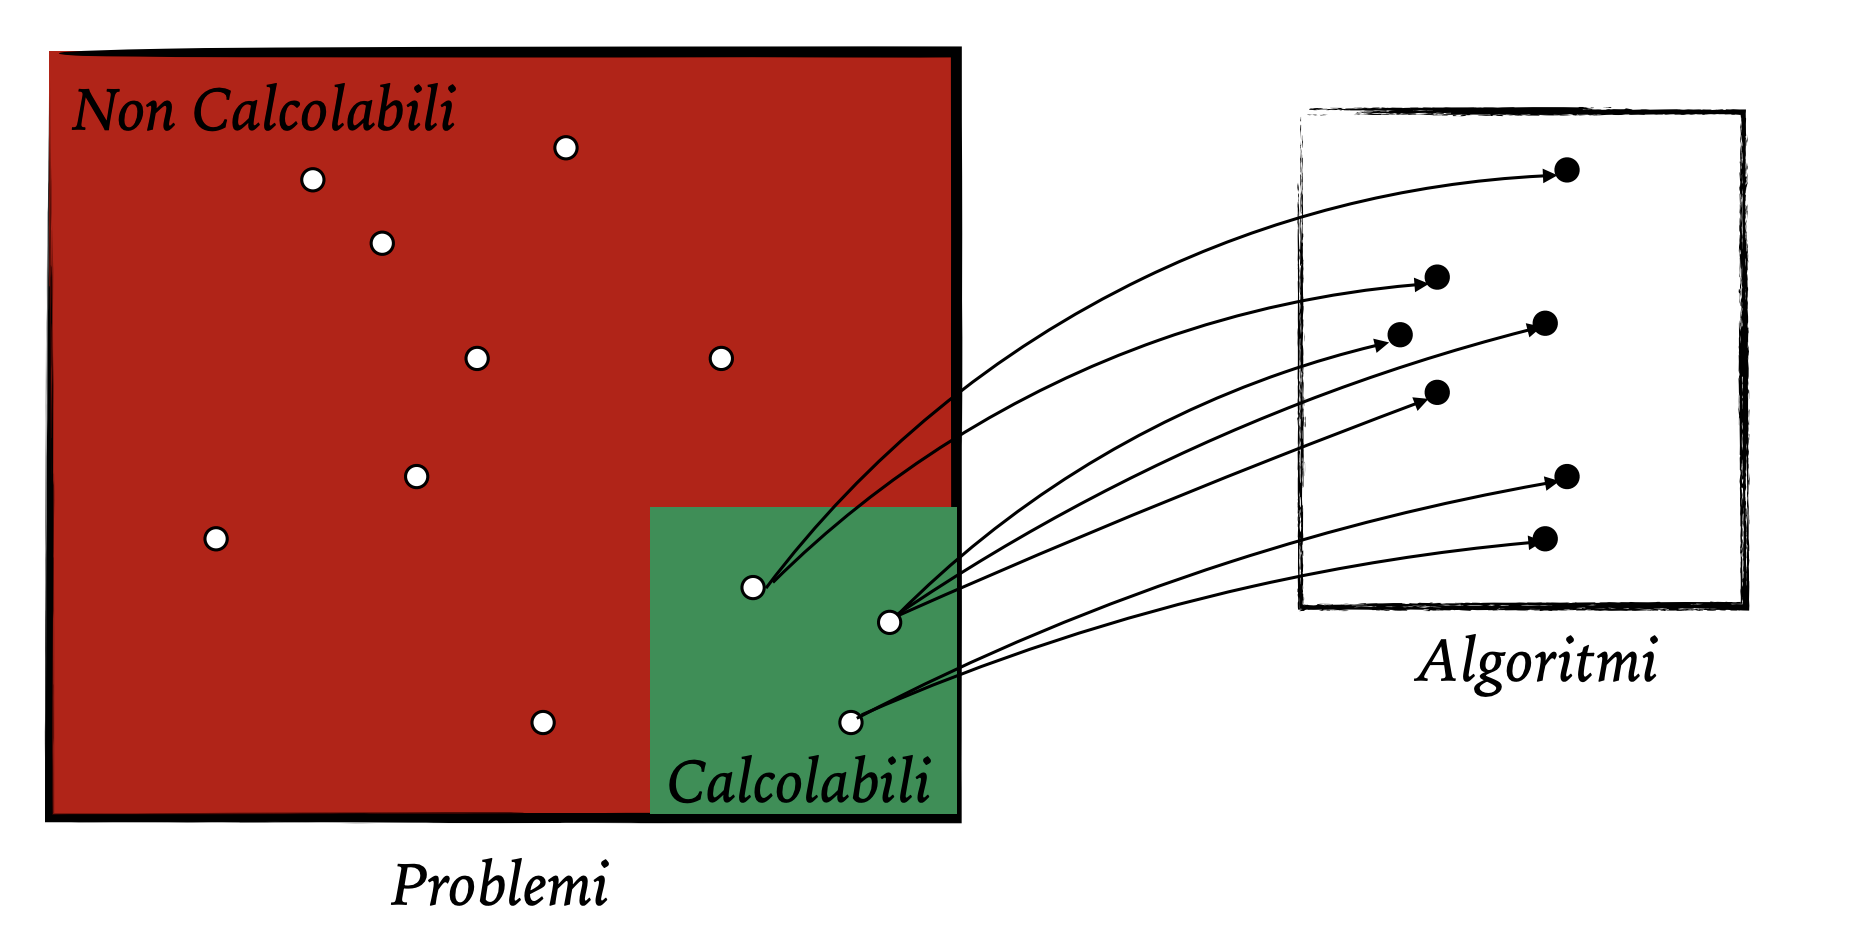
\includegraphics[width=0.9\textwidth]{fcalcolabili.png}
\end{figure}

\section{Principio di induzione}

Il principio di induzione ha senso solo su insieme infiniti 
e serve per dimostrare che una proprietà vale per tutti gli elementi.
Esistono due metodi di induzione:
\begin{itemize}
    \item Induzione matematica
    \item Induzione strutturale
\end{itemize}
Tratteremo nello specifico caso in questo corso \textbf{l'induzione matematica.}
Partiamo da un insieme $A$ infinito con una relazione $< \; : (A, <)$ è una relazione d'ordine
non riflessiva perché non è minore stretto.
Utilizziamo l'induzione matematica e quindi $A = \mathbb{N}$ e $<$ 
è l'ordinamento stretto tra numeri. Una relazione d'ordine deve essere
\textit{ben fondata} vuol dire che non esistono catene discendenti infinite.
Una catena discendente è una sequenza infinita di elementi
\[a_0 > a_1 > a_2 > a_3 > \dots\]
In un tipo di relazione riflessiva è sicuramente non ben fondata perché posso fare 
continuare ad inserire lo stesso numero all'infinito.
\[m \text{ minimale in } A \; : \; b \in A \text{ è minimale se } \forall b' < b . b' \notin A\]
\ex{}
{
    Se prendiamo $\{1,2,3\}$ con relazione d'ordine di contenimento
    allora esistono più minimali come $\{1,2\}$ o $\{2,3\}$. 
    Quindi se $A = \mathbb{N} \Longrightarrow \exists b $ minimo $\forall x \subseteq \mathbb{N}$. 
}
\noindent
Quindi preso $A$ insieme ben fondato con ordinamento $<$ allora:
$\pi$ proprietà definita sugli elementi di \[
A: \pi \subseteq A \text{ allora } 
\forall a \in A \, .\pi(a) \Longleftrightarrow \forall a \in A . [[\forall b < a . \pi(b)] \rightarrow \pi(a)]
\]
Se dimostriamo $\pi$ per ogni elemento più piccolo di $a$ allora $\pi$ vale per $a$.
\[{Base}_A = \{a \in A | a \text{ minimale}\}\]
Quindi
\[\overbrace{\forall A \in {Base}_A \; . \; \pi(a)}^{\text{Base}} \; \and \; 
\underbrace{\forall a \in A . {Base}_A}_{\text{passo induttivo}} . \overbrace{\forall b < a . \pi(b)}^{\text{ipotesi induttiva}} \rightarrow \underbrace{\pi(a)}_{\text{tesi}}
\]
\ex{}
{
    Prendiamo come esempio il seguente enunciato:
    \[\forall n \in \mathbb{N}, \; \;  \sum_{i = 1}^{n} i = \frac{n(n+1)}{2}\]
    \textbf{Base:} $n=1$
    \[A = \mathbb{N} \backslash \{0\} \; \; {Base}_A = \{1\} \rightarrow \sum_{i=1}^{1} i = 1\]
    \[
    \begin{aligned}
        \sum_{i=1}^{1} i &= 1\\
        &= n(n+1)/2\\
        &= \frac{1(1+1)}{2} = 1\\
    \end{aligned}    
    \]
    Caso base dimostrato.\\
    \textbf{Passo induttivo:} prendo $n \in \mathbb{N}$ e applico l'ipotesi induttiva: per ogni $k < n$ vale la tesi.
    \[\text{ Tesi da dimostrare: } \sum_{i=1}^{n} i = \frac{n(n+1)}{2}\]
    \[\sum_{i=1}^{n} i = \sum_{i=1}^{n-1}i + n\]
    Sappiamo sicuramente che $n-1 < n$ e per ipotesi induttiva:
    \[\sum_{i=1}^{n-1}i + n= \frac{(n-1)(n-1+1)}{2} + n = \frac{n(n-1)}{2} + n = \]
    \[\frac{n(n-1) + 2n}{2} = \frac{n(n-1+2)}{2} = \frac{n(n+1)}{2} \quad \square\] 
    e quindi la tesi vale perché siamo arrivati alla stessa espressione
    che volevamo dimostrare.
}
\subsection{Linguaggi formali}
\dfn{Linguaggio formale}
{
    Un linguaggio formale è un insieme di stringhe composte da simboli in un alfabeto finito $\Sigma$.
}
\noindent
$\Sigma^*$ denota il linguaggio di tutte le stringhe dell'alfabeto $\Sigma$, se $\Sigma$ non è vuota allora $\Sigma^*$ è 
infinito e numerabile.
Solitamente un linguaggio formale $\mathcal{L}$ è un sottoinsieme di $\Sigma^*$ tipicamente infiniti ma non è necessario:
\[\mathcal{L} \subseteq \Sigma^*\]
I linguaggi finiti sono sicuramente regolari perché \textit{posso sempre costruire un automa a stati finiti} che li riconosce.

\begin{figure}[H]
    \centering
    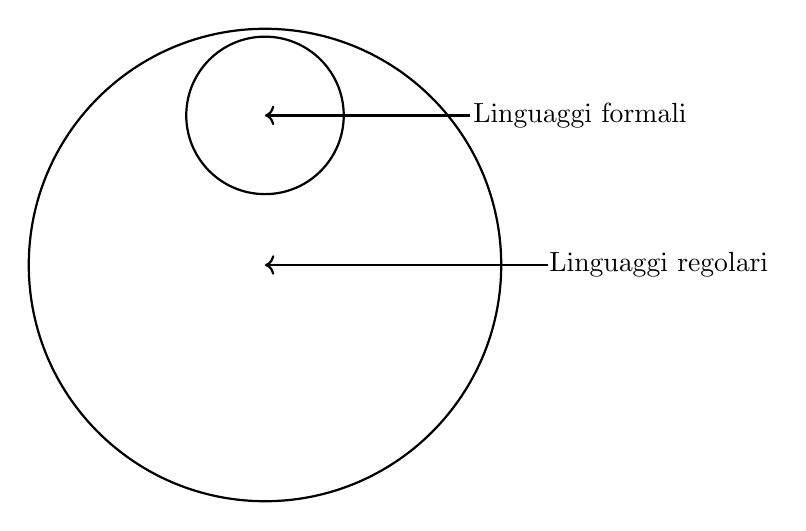
\begin{tikzpicture}
        \draw[thick] (0,0) circle(3);
        \draw[thick] (0,1.9) circle(1);
        \node at (4,1.9) {Linguaggi formali};
        \draw[<-, thick] (0,1.9) -- (2.6,1.9);
    
        \node at (5,0) {Linguaggi regolari};
        \draw[<-, thick] (0,0) -- (3.6,0);
      \end{tikzpicture}
\end{figure}


\begin{figure}[H]
    \centering
    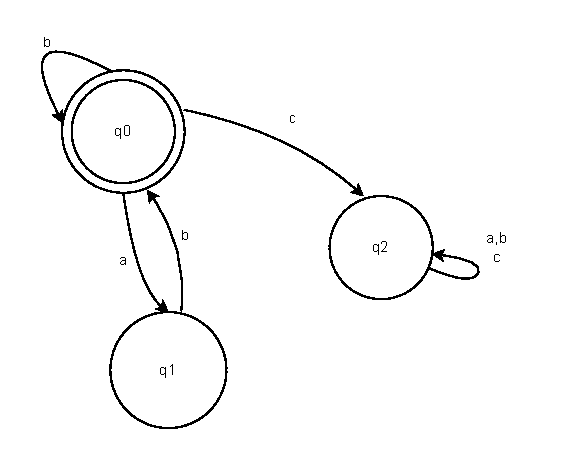
\includegraphics[width=0.6\textwidth]{automa.pdf}
    \caption{Esempio di automa a stati finiti}
\end{figure}
\end{document}